\section{Associated Files}\label{associated-files}

Three files come with the auxiliary view factor package. They are:

\begin{itemize}
\item
  View3D.exe
\item
  ViewFactorInterface.xls
\item
  View3D32.doc
\end{itemize}

The first is the executable program that calculates the view factors. The second is an excel interface that will set up the input files and execute View3D.exe. The third file is the documentation file from NIST that contains some explanation of the program.

\section{Using the View Factor Interface program}\label{using-the-view-factor-interface-program}

The interface program has two main sheets. One, named ZoneSheet, uses surface areas, tilts and facing directions to develop the input for View3D. The other one, named VerticesZoneSheet, uses the surface vertices to develop the input for View3D. The sheets are shown in Figure~\ref{fig:view-factor-interface-zonesheet} and Figure~\ref{fig:view-factor-interface-verticeszonesheet}.

\begin{figure}[hbtp] % fig 24
\centering
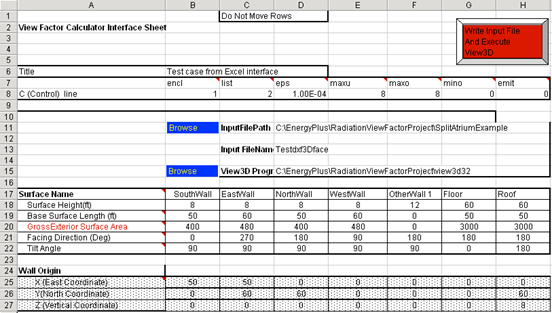
\includegraphics[width=0.9\textwidth, height=0.9\textheight, keepaspectratio=true]{media/image022.png}
\caption{View Factor Interface ZoneSheet \protect \label{fig:view-factor-interface-zonesheet}}
\end{figure}

\begin{figure}[hbtp] % fig 25
\centering
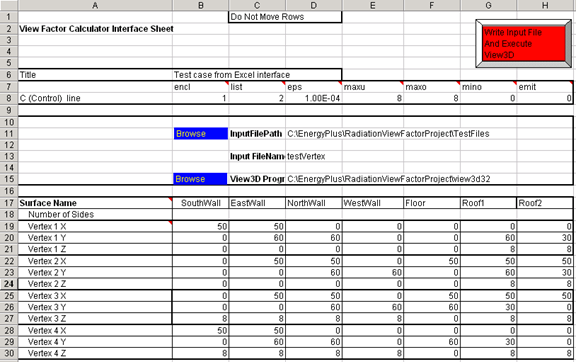
\includegraphics[width=0.9\textwidth, height=0.9\textheight, keepaspectratio=true]{media/image023.png}
\caption{View Factor Interface VerticesZoneSheet \protect \label{fig:view-factor-interface-verticeszonesheet}}
\end{figure}

Either sheet can be used to generate an input file for the View3D program. An example of that file is shown below.

\begin{lstlisting}
T Test case from Excel interface
C encl =  1  list =  2  eps =  0.0001  maxu =  8  maxo =  8  mino =  0  emit =  0
F  3
V  1  50  0  0
V  2  0  0  0
V  3  0  0  8
V  4  50  0  8
S  1  1  2  3  4   0  0   .999  SouthWall
! = = = = = = = = = = = = = = = = = = = = = = = = =
V  5  50  60  0
V  6  50.00025  0  0
V  7  50.00026  0  8
V  8  50.00001  60  8
S  2  5  6  7  8   0  0   .999  EastWall
! = = = = = = = = = = = = = = = = = = = = = = = = =
V  9  0  60  0
V  10  50  60.00014  0
V  11  50  60.00015  8
V  12  0  60.00001  8
S  3  9  10  11  12   0  0   .999  NorthWall
! = = = = = = = = = = = = = = = = = = = = = = = = =
V  13  0  0  0
V  14  0  60  0
V  15  0  60  8
V  16  0  0  8
S  4  13  14  15  16   0  0   .999  WestWall
! = = = = = = = = = = = = = = = = = = = = = = = = =
V  17  0  0  0
V  18  50  1.377901E-04  0
V  19  49.99984  60.00014  0
V  20 -1.653482E-04  60  0
S  5  17  18  19  20   0  0   .999  Floor
! = = = = = = = = = = = = = = = = = = = = = = = = =
V  21  0  60  8
V  22  50  60.00014  8
V  23  50.00016  1.373291E-04  8.000166
V  24  1.653482E-04  0  8.000166
S  6  21  22  23  24   0  0   .999  Roof
! = = = = = = = = = = = = = = = = = = = = = = = = =
End Of Data
\end{lstlisting}

Notice the title from row 6 on the interface appears at the top of the input file, and the control line information in rows 7 and 8 appear below the title line in a line with the character C at the left end. The explanation of the control parameters from the program document states:

(C c) The control line includes the following parameters (in order): name = value

eps = 1.0e-4

integration convergence criterion for both adaptive integration and view obstruction. This is not an exact measure of the accuracy of the computed view factors, but smaller values will usually lead to more precise values. The convergence criteria should not be less than about 1.0e-6 because many of the intermediate calculations are accurate only to single (32-bit) precision.

maxU = 8

maximum recursions used in computing the unobstructed view factors.

maxO = 8

maximum recursions used in computing the obstructed view factors. Limiting the maximum number of recursions limits the total execution time of the program but may prevent reaching the specified convergence.

minO = 0

minimum recursions: used in computing the obstructed view factors. This can help in cases where an obstruction occurs very near the view between the edges of two surfaces. The normal adaptive integration may miss the obstruction. Increasing this value from its normal value of 0 to 1 or 2 may catch the obstruction. This is probably not necessary except when very accurate view factors are desired. It can add considerably to execution time.

row = 0

selected row for computing view factors (0 = all rows)

col = 0

selected column for computing view factors (0 = all columns)

encl = 0

1 indicates that the surfaces form an enclosure; 0 indicates that they do not. This data is used to adjust the view factors of an enclosure to guarantee conservation of energy.

emit = 0

1 indicates that diffuse reflectance effects will be included in the computed view factors; 0 indicates they will not, i.e., surfaces will be considered `black'.

out = 0

view factor output file format - 1 = \ldots{}gence criterion for the numerical integration used to compute view factors between surfaces that have view obstructing surfaces between them.

list = 0

computational summary written to the VIEW3D.LOG file; 0 gives minimal information; 1 gives slightly more; 2 prints all the view factors; 3 causes dumping of some intermediate values.

The values of the parameters shown on the interface sheets are reasonable defaults, and they should need to be adjusted only rarely.

In the upper right corner of either sheet is a button that causes two files to be generated and View3D to be executed. The two files generated are the input file that uses the name from cell D13 with the extension vs3, and a file with the same name and an extension dxf. VoloView can be used with this file to generate a wire frame drawing of the zone being analyzed.

Two paths are needed for executing the program. The directory path where the vs3 and dxf files will be placed is specified in cell D11. This directory can be selected using the Browse button in cell B11. The path to the View3D.exe program is specified by cell D15. This directory can be selected with the Browse button in cell B15.

If you are using the ZoneSheet, the zone surfaces are described in the region from row 17 to row 27. Each column supplies the details for one surface. Additional surface columns can be added by copying and pasting a desired starting column to the right of column H. If either the surface height or base surface length is zero, the gross area cell will be zero and column is ignored. The facing direction of the surface is the direction an inward normal to the surface would point. So, the south wall of a zone faces north or 0 degrees. Note that this is different from EnergyPlus where the facing direction of a surface is based on the outward normal. The facing direction becomes just slightly more difficult with horizontal surfaces like floors and ceilings. The key to determining their facing direction is to visualize them being rotated slightly into the zone around their base surface axis. In the example, both ceiling and floor are chosen to face south. The tilt of a surface is relative to a horizontal upward facing (in the conventional sense) surface such as a floor. A ceiling or flat roof it tilted 180 degrees. Vertical surfaces have a tilt of 90 degrees.

The remaining information needed to describe the surfaces is the coordinates of the lower left hand corner of the surface when viewed from inside the zone. This is where the visualization of a slight rotation of the floor and roof becomes helpful. Consider the roof surface on the sheet. Its base side lies along the east west axis since it faces south. With a slight inward rotation, it is clear that the lower left hand corner is the northwest corner of the roof. This corner has coordinates of 0, 60, and 8.

If the VerticesZoneSheet is being used, the description of the surfaces consists only of the vertices. For this program, the vertices are specified in a counter clockwise rotation order if looking at the surface from the inside, and in a clockwise rotation order if looking from the outside.

The vs3 file produced is shown previously and the dxf file generates the wire frame drawing shown in Figure~\ref{fig:dxf-format-of-example-zone}.

\begin{figure}[hbtp] % fig 26
\centering
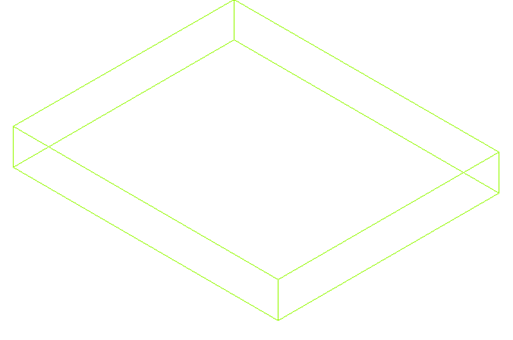
\includegraphics[width=0.9\textwidth, height=0.9\textheight, keepaspectratio=true]{media/image024.png}
\caption{DXF Format of Example Zone \protect \label{fig:dxf-format-of-example-zone}}
\end{figure}

The input file and the output files produced by View3D are read into the interface spreadsheet, and appear on new worksheets.

Figure~\ref{fig:files-brought-into-the-interface-workbook} shows the lower corner of the interface sheet with the additional sheet tabs.

\begin{figure}[hbtp] % fig 27
\centering
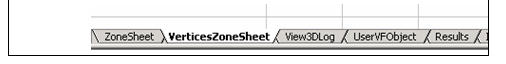
\includegraphics[width=0.9\textwidth, height=0.9\textheight, keepaspectratio=true]{media/image025.png}
\caption{Files brought into the Interface Workbook \protect \label{fig:files-brought-into-the-interface-workbook}}
\end{figure}

The results file is named with the name in cell D13 with an extension of out. This file is shown below.

\begin{lstlisting}
View3D 3.2 0 1 0 6
400 480 400 480 3000 3000
0.000000 0.078244 0.029324 0.078217 0.407109 0.407106
0.065204 0.000000 0.065204 0.044282 0.412652 0.412659
0.029324 0.078245 0.000000 0.078217 0.407110 0.407105
0.065181 0.044282 0.065181 0.000000 0.412679 0.412677
0.054281 0.066024 0.054281 0.066029 0.000000 0.759385
0.054281 0.066025 0.054281 0.066028 0.759385 0.000000
0.999 0.999 0.999 0.999 0.999 0.999
\end{lstlisting}

Excel macro capabilities are used by the interface to convert the text to columns and add the surface names and other headings. The modified results are placed on the Results worksheet as shown in Figure~\ref{fig:view-factors-with-surface-names-inserted}.

\begin{figure}[hbtp] % fig 28
\centering
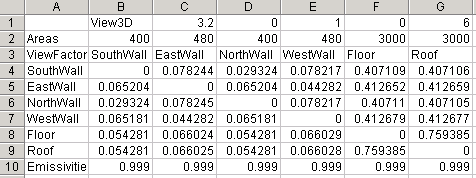
\includegraphics[width=0.9\textwidth, height=0.9\textheight, keepaspectratio=true]{media/image026.png}
\caption{View Factors with Surface Names Inserted \protect \label{fig:view-factors-with-surface-names-inserted}}
\end{figure}

The results file information is used to generate a UserViewFactor object for EnergyPlus. This object is located in the first column of a new worksheet named UserVFObject. This column can simply be copied and inserted into the EnergyPlus idf file.

If the results sheet does not appear, or the program terminates, the sheet named View3Dlog or the output file by the same name should be consulted. It contains a complete history of the execution. Any problem with the input file or the calculations should show up there.

The extra sheets generated by the VBA macros will be deleted if the program is called with the run button while they are present. The user will be queried to make sure the sheets should be deleted. During the succeeding run, new sheets will be created.
